\chapter{Deus et Eliseus Ascenderunt in Caelum}
\begin{center}
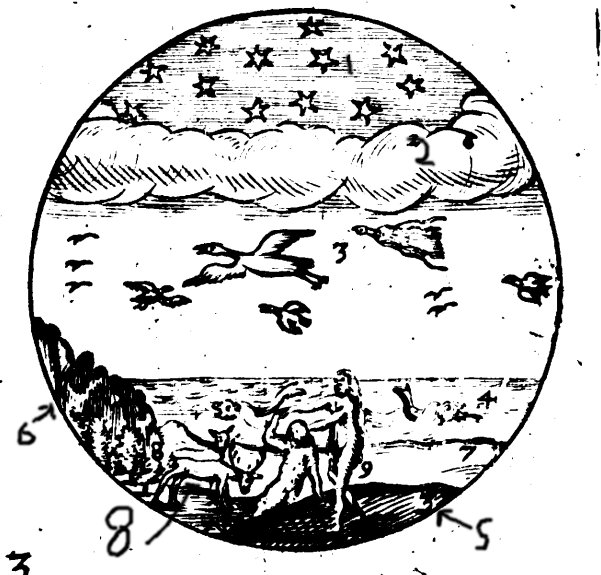
\includegraphics[scale=1.5]{World.png}
\end{center}

\section{Intended Audience}
This is intended for students who have completed Lectio 3 and 4 of Latin by the Natural Method and Chapter 4 of Lingua Latina Per Se Illustrata. 

\section{Text}
Deus et Eliseus filius meus parvus ascenderunt in Caelum. Quomodo Deus ascendit in caelum, si sine corpore et sine loco est? Deus incarnationem habet, qui ascendit in caelum et descendit ex caelo. Incarnatio secundi hypostasis trinitatis est Iesus Christus. Ergo, Deus (in incarnatione) et Eliseus fuerunt in nubibus, quia ascenderunt in Caelo. Elias etiam et Iesus ascenderunt in caelum, sed Iesus solus sedet ad manum dexteram Dei. 

In Caelo, Eliseus vidit aves, quae volaverunt per nubes. Ubiubi Avis volavit, movet aerem. Ubiubi Eliseus aspexit, Eliseus vidit aves et nubes. Quid non vidit Eliseus? Angelos non vidit Eliseus. Cur? Estne Angeli in Caelo cum Deo? Ita, sed Caelum habet duas significationes. Significatio prima est haec \: Ubi sunt nubes et aves et sol et luna. Significatio secunda \: Ubi sunt Angeli. Angeli non habent corpora nec locos, sicut Deus in essentia. Sed angeli in Caelo sunt


\footnote{\textbf{Montēs} = Montains or Hills}